%%===========================================================%%
%%                                                           %%
%%          TPC TRACK POINTING RESOLUTION ADJUSTMENT         %%
%%                                                           %%
%%===========================================================%%


\chapter{TPC track pointing resolution adjustment}\label{chap:tpcTrackPointingRes}

It was found during the analysis that distributions of quantities which describe the pointing resolution of the TPC tracks do not agree well between the data and embedded MC. Namely, the resolutions of the global helices associated with the tracks were found to be significantly better in the STAR simulation than in the data, what manifests as narrower DCA and $d_{0}$ distribution in the embedded MC, comparing to corresponding distribution in the data (Fig.~\ref{fig:pointingResComp}). This issue was discussed under ticket \#3332~(Ref.~\cite{dcaTicket}).

This problem could affect the momentum resolution and thus all other resolutions and reponse matrices used in data unfolding. Therefore the resolution adjustment procedure was performed to find appropriate parameters of the ``artificial'' helix deterioration and finally obtain agreement between DCA and $d_{0}$ distributions (and all related resolutions) in the data and embedded MC.

In order to reduce pointing resolution in the MC an additional smearing of the helix radius $\sigma(R)$ was introduced. Based on $d_{0}$ comparison in~Fig.~\ref{fig:d0} it was decided to account also for the systematic bias of the helix radius $\Delta\mu(R)$\footnote{Transverse impact parameter $d_{0}$ takes positive value if the beamline is contained inside the helix (in the $yz$-plane projection), otherwise it is negative. Any asymmetry in the $d_{0}$ distribution in the MC with respect to the data indicates presence of systematic difference in reconstructed $d_{0}$, hence also in reconstructed $R$.}, which may be present e.g. due to differences in the material budget used the simulation and reconstruction. Both smearing and bias of the helix radius were introduced only for MC tracks which were matched with the true-level particles since only simulated tracks require adjustment (tracks from zero-bias event used in embedding already contain all detector effects).

%---------------------------
\begin{wrapfigure}{i}{0.365\textwidth}\vspace*{-9pt}
  \centering
  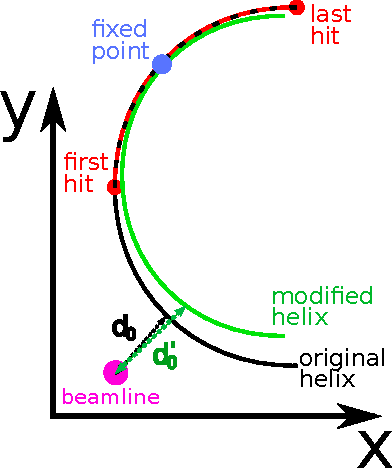
\includegraphics[width=0.365\textwidth]{graphics/tpcHelixAdj/trackSmearing.pdf}
  \caption[Sketch of helix modification procedure and $d_{0}$ calculation.]
   {Sketch of helix modification procedure and $d_{0}$ calculation.}
   \label{fig:d0sketch}%\vspace*{-29pt}
\end{wrapfigure}
%---------------------------

Extraction of $\Delta\mu(R)$ and $\sigma(R)$ parameter required to achieve agreement of pointing resolution between embedded MC and the data involved a few steps, as listed below:
  \begin{enumerate}
   \item Series of $d_{0}$ histograms in bins of $p_{T}$ (100~MeV/$c$ wide) was prepared, each for different size of distortion (different $\Delta\mu(R)$ and $\sigma(R)$) of global helix of the TPC tracks matched with true-level particles (example plot in single $p_{T}$ bin is shown in Fig.~\ref{fig:d0ForChiSqMin}):
   \begin{enumerate}
   \item for each set of parameters $\Delta\mu(R)$ and $\sigma(R)$ the helix radius $R$ was recalculated independently for each track following the Eq.~\eqref{eq:radiusRecalc}:\vspace{-5pt}
   \begin{equation}\label{eq:radiusRecalc}R'=R\times \mathcal{N}\Big(1+\Delta\mu(R),~\sigma(R)\Big),\vspace{-5pt}\end{equation}
   \item new helix of a radius $R'$ was assigned to a track and used to calculate $d_{0}$. The modified helix was obtained by changing the radius of original helix from $R$ to $R'$ with a fixed middle point between the first and last TPC hit of a global track represented by the helix (Fig.~\ref{fig:d0sketch}). The momentum of the track was also recalculated:\vspace{-5pt}
   \begin{equation}p_{T}'=p_{T}\times \frac{R'}{R},~~~~~~~\eta'=\eta\times \frac{R'}{R}.\vspace{-5pt}\end{equation}
   \end{enumerate}%
  \end{enumerate}%
 
  \begin{enumerate}\setcounter{enumi}{1}
   \item In each $p_{T}$ bin the $\chi^{2}/\text{NDF}$ was calculated between the data and MC $d_{0}$ histogram in a range -1.5~cm~$<d_{0}<$~1.5~cm (corresponding to $d_{0}$ cut used in analyses), for every point in parameter space of radius distortion (for every set of $\Delta\mu(R)$ and $\sigma(R)$). An example (single $p_{T}$ bin) of map of $-\chi^{2}/\text{NDF}$ in a~parameter space is presented in~Fig~\ref{fig:chiSqPerNdfTpcResAdj}.
   \item In each bin of recalculated $p_{T}$ the 2-dim parabola $z\left(x,y;~a,b,x_{0},y_{0},z_{0}\right)$ given in Eq.~\eqref{eq:parabolaChiSq} ($z=\chi^{2}/\text{NDF},~x=\Delta\mu(R),~y=\sigma(R)$) was fitted to $-\chi^{2}/\text{NDF}$ in the global minimum region to obtain the best-fit distortion parameters.\vspace{-5pt}
   \begin{equation}\label{eq:parabolaChiSq}  z=z_{0}-a(x-x_{0})^{2}-b(y-y_{0})^{2}.\vspace{-5pt}\end{equation}
   \item The best-fit smearing $\sigma(R)$ (equal to parabola parameter $y_{0}$) and best-fit bias $\Delta\mu(R)$ ($x_{0}$) from individual $p_{T}$ bins was plotted as a function of global track $p_{T}$ (Fig.~\ref{fig:distortionVsPt}). Each point was assigned with an error being a quadratic sum of two components: the error on $x_{0}$ ($y_{0}$) resulting from the parabola fit to $-\chi^{2}/\text{NDF}$, and length of corresponding semi-axis of ellipsis formed by the intersection of fitted parabola with the $xy$-plane at $z=z_{0}-1/\text{NDF}$ (from definition of the parameter uncertainty given by the change of overall $\chi^{2}$ by 1 unit). Resultant formulae for the error of each individual point in Fig.~\ref{fig:distortionVsPt} are%\vspace{-5pt}
   \begin{multicols}{2}~\\[-30pt]
    \begin{equation}\label{eq:errorDeltaMuR}  \delta\left(\Delta\mu(R)\right)=\sqrt{\delta_{\text{fit}}^{2}(x_{0}) + \frac{1}{2a\text{NDF}}},\end{equation}
   \break\\[-60pt]
    \begin{equation}\label{eq:errorSigmaR} \delta\left(\sigma(R)\right)=\sqrt{\delta_{\text{fit}}^{2}(y_{0}) + \frac{1}{2b\text{NDF}}}.\vspace{-5pt}\end{equation}
    \end{multicols}\vspace*{-7pt}
    From Fig.~\ref{fig:d0ForChiSqMin} one can read that $\text{NDF}=14$. In calculation of uncertainties correlation of $\Delta\mu(R)$ and $\sigma(R)$ have not been accounted.
   \item The empirically determined functions were fitted to points representing $\Delta\mu(R)$ and $\sigma(R)$ dependence on the global track $p_{T}$. Their form and values of parameters are given in Fig.~\ref{fig:distortionVsPt}.
  \end{enumerate}%
  
%---------------------------
\begin{figure}[t!]%
\centering%
\begin{minipage}{.4725\textwidth}%
  \centering%
  \includegraphics[width=\linewidth,page=5]{graphics/tpcHelixAdj/D0ComparisonForChiSqMinimization.pdf}%
  \caption[Example of comparison of $d_{0}$ histograms in the data and embedded MC in the procedure of TPC pointing resolution adjustment.]{Example of comparison of $d_{0}$ histograms in single $p_{T}$ bin in the data (black points) and embedded MC (colored lines) in the procedure of TPC pointing resolution adjustment. MC histograms only for $\Delta\mu(R)=0$ and $\sigma(R)=0$, $5\times10^{-3}$ and $10^{-2}$ were shown for explanatory purposes.}\label{fig:d0ForChiSqMin}
\end{minipage}%
\quad\quad%
\begin{minipage}{.4725\textwidth}%
  \centering
  \includegraphics[width=\linewidth,page=3]{graphics/tpcHelixAdj/ChiSqVsSmearingVsBias.pdf}%
  \caption[Example of $-\chi^{2}/\text{NDF}$ map in a parameter space in the procedure of TPC pointing resolution adjustment.]{Example of $-\chi^{2}/\text{NDF}$ map in a parameter space in the procedure of TPC pointing resolution adjustment. The red surface represents parabola fitted in the vicinity of the global minimum.\newline\newline}\label{fig:chiSqPerNdfTpcResAdj}
\end{minipage}%
\end{figure}%
%---------------------------

  
%---------------------------
\begin{wrapfigure}{o}{0.465\textwidth}\vspace*{-15pt}
  \centering
  ~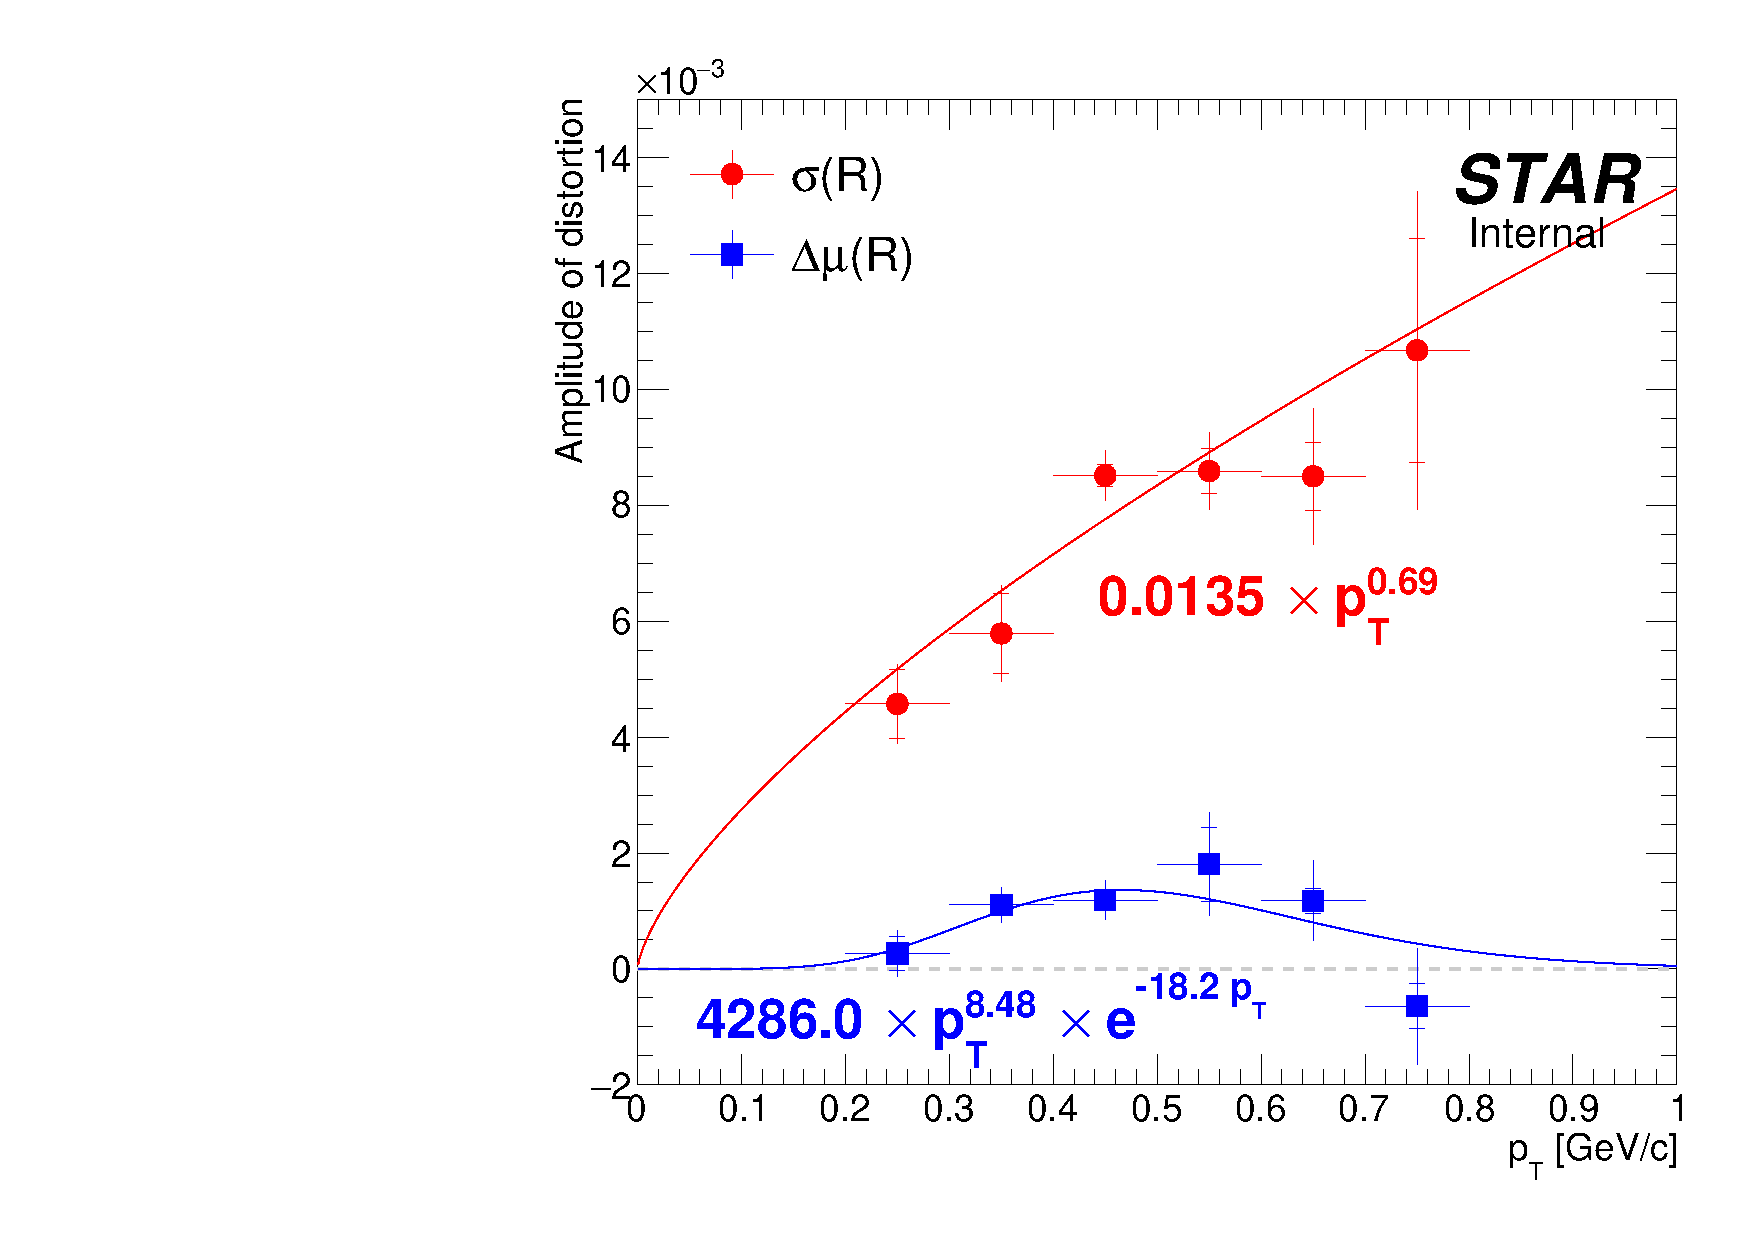
\includegraphics[width=0.465\textwidth]{graphics/tpcHelixAdj/DistortionVsPt.pdf}\vspace*{-5pt}
  \caption[Best-fit parameters obtained in the procedure of the TPC track pointing resolution adjustment.]
   {Best-fit parameters obtained in the procedure of the TPC track pointing resolution adjustment. Uncertainties on parameters resulting solely from the fit of Eq.~\eqref{eq:parabolaChiSq} to $-\chi^{2}/\text{NDF}$ are represented by the lines with perpendicular endings. Total uncertainties (Eqs.~\eqref{eq:errorDeltaMuR},~\eqref{eq:errorSigmaR}) extend beyond. The empirical functions fitted to points are drawn with corresponding colors, and formula of each is written aside.}
   \label{fig:distortionVsPt}%\vspace*{-29pt}
\end{wrapfigure}
%---------------------------
Helices of global TPC tracks were deteriorated according to Eq.~\eqref{eq:radiusRecalc} and the parametrizations of global track $p_{T}$-dependence of $\Delta\mu(R)$ and $\sigma(R)$ from Fig.~\ref{fig:distortionVsPt}, to verify if better agreement between the data and embedded MC is found after the adjustment. Filled histograms in Fig.~\ref{fig:pointingResComp} show $d_{0}$ and DCA distributions after the described adjustment, and filled circles in the bottom pad show their ratio to the data points. Clearly, there is much better agreement between embedded MC and the data after the pointing resolution adjustment. Remaining differences may arise from incomplete theoretical model of the CEP process impleneted in GenEx leading to different $p_{T}$ spectra of the data and the model (e.g. model does not contain resonant $\pi^{+}\pi^{-}$ production).





%---------------------------
\begin{figure}[ht]
\centering
\parbox{0.4725\textwidth}{
  \centering
  \begin{subfigure}[b]{\linewidth}
                \subcaptionbox{\label{fig:d0}}{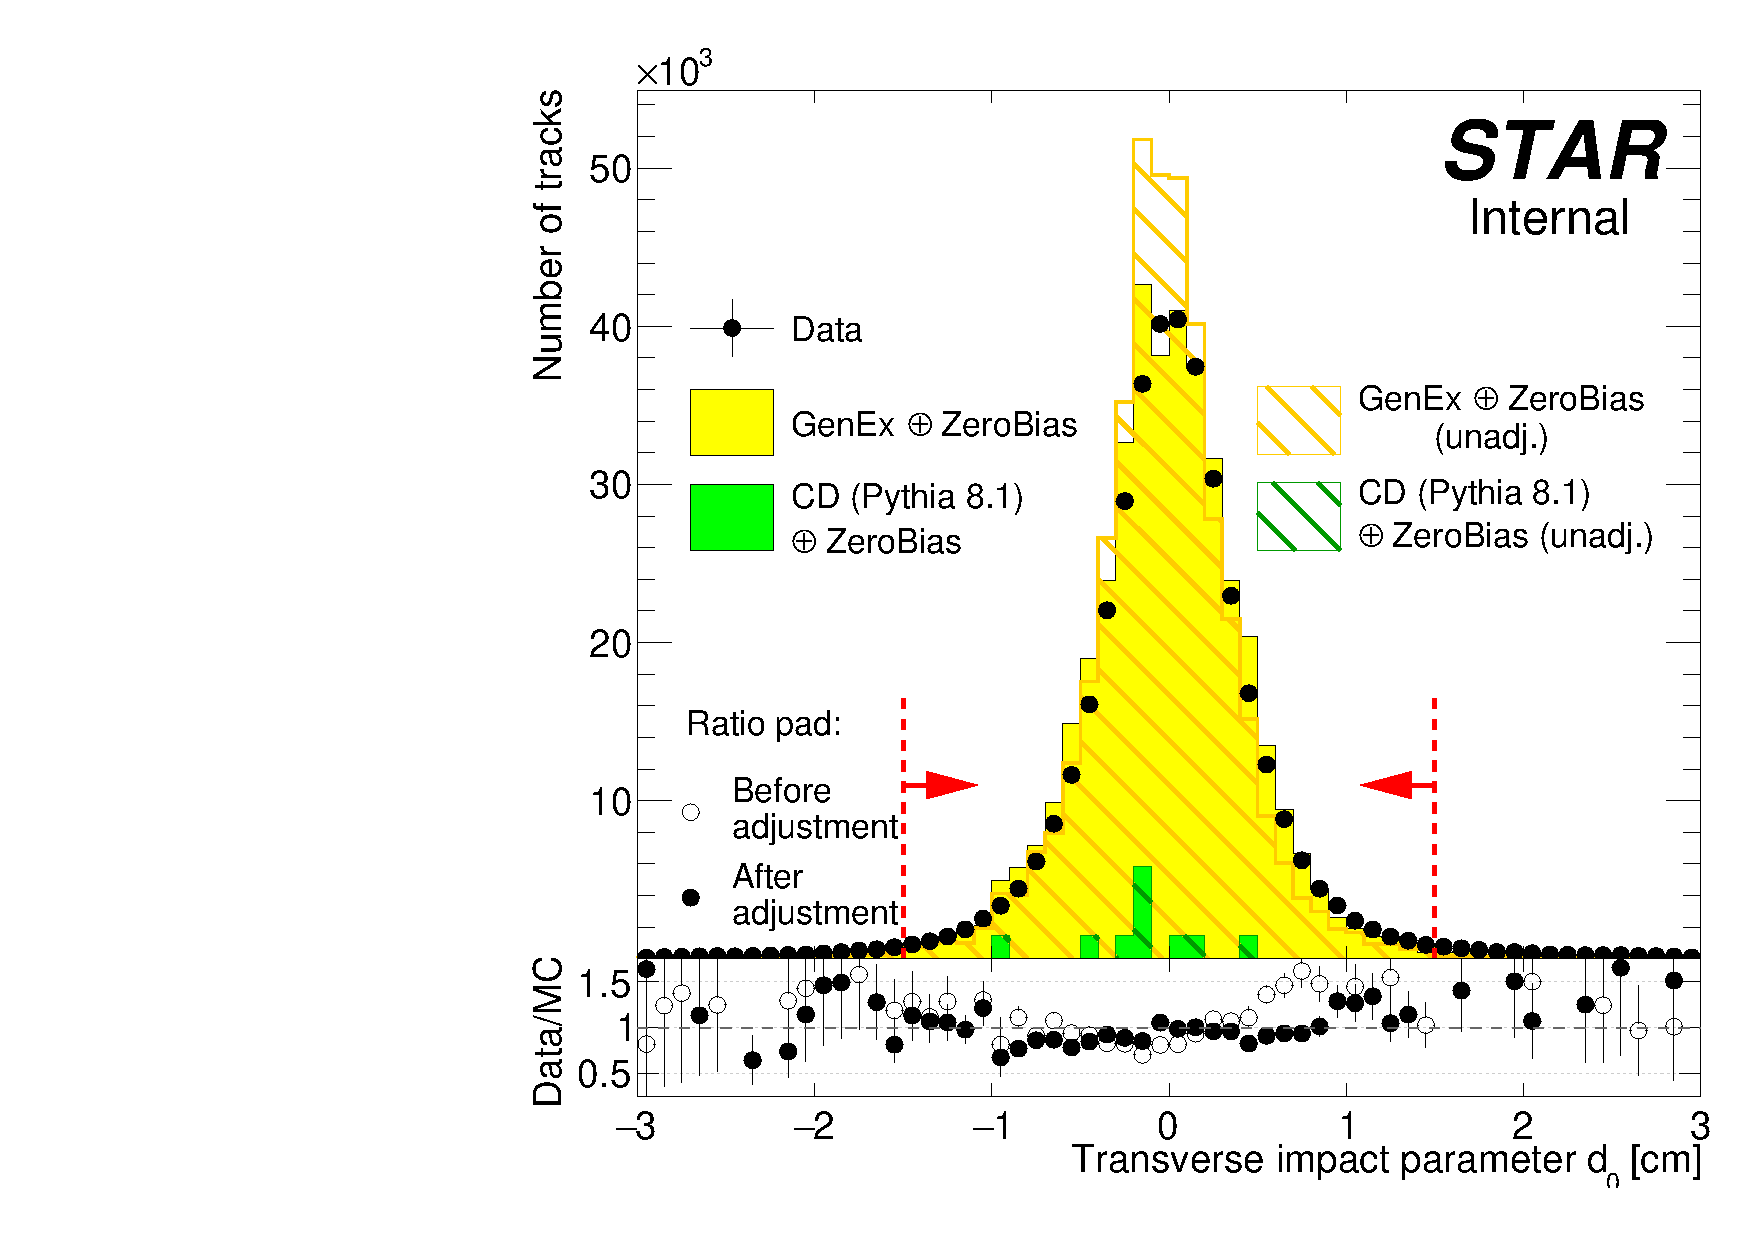
\includegraphics[width=\linewidth]{graphics/tpcHelixAdj/d0_beforeAfterCorrection.pdf}}
  \end{subfigure}\\
  \begin{subfigure}[b]{\linewidth}\addtocounter{subfigure}{1}
                \subcaptionbox{\label{fig:dcaX}}{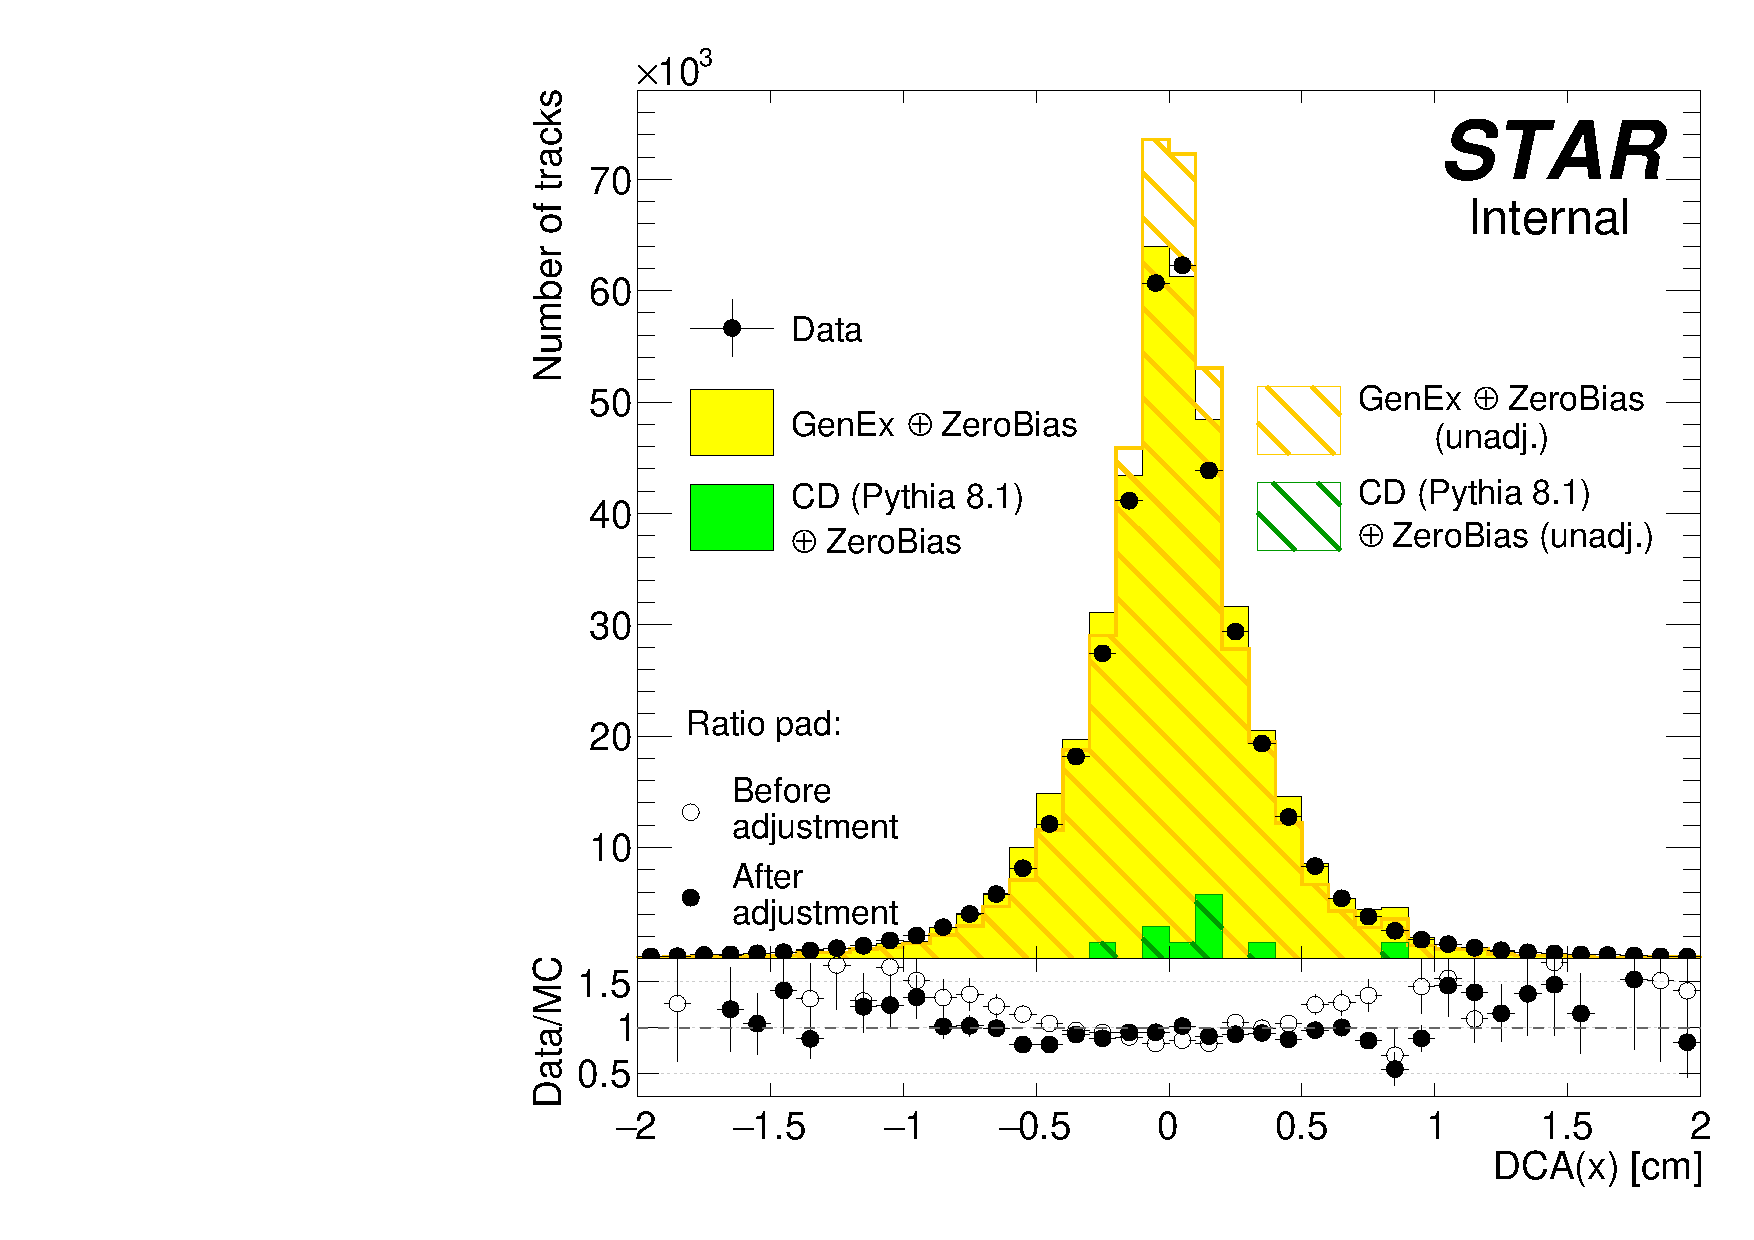
\includegraphics[width=\linewidth]{graphics/tpcHelixAdj/DcaX_beforeAfterCorrection.pdf}}
  \end{subfigure}\\
  \begin{subfigure}[b]{\linewidth}\addtocounter{subfigure}{1}
                \subcaptionbox{\label{fig:dcaZ}}{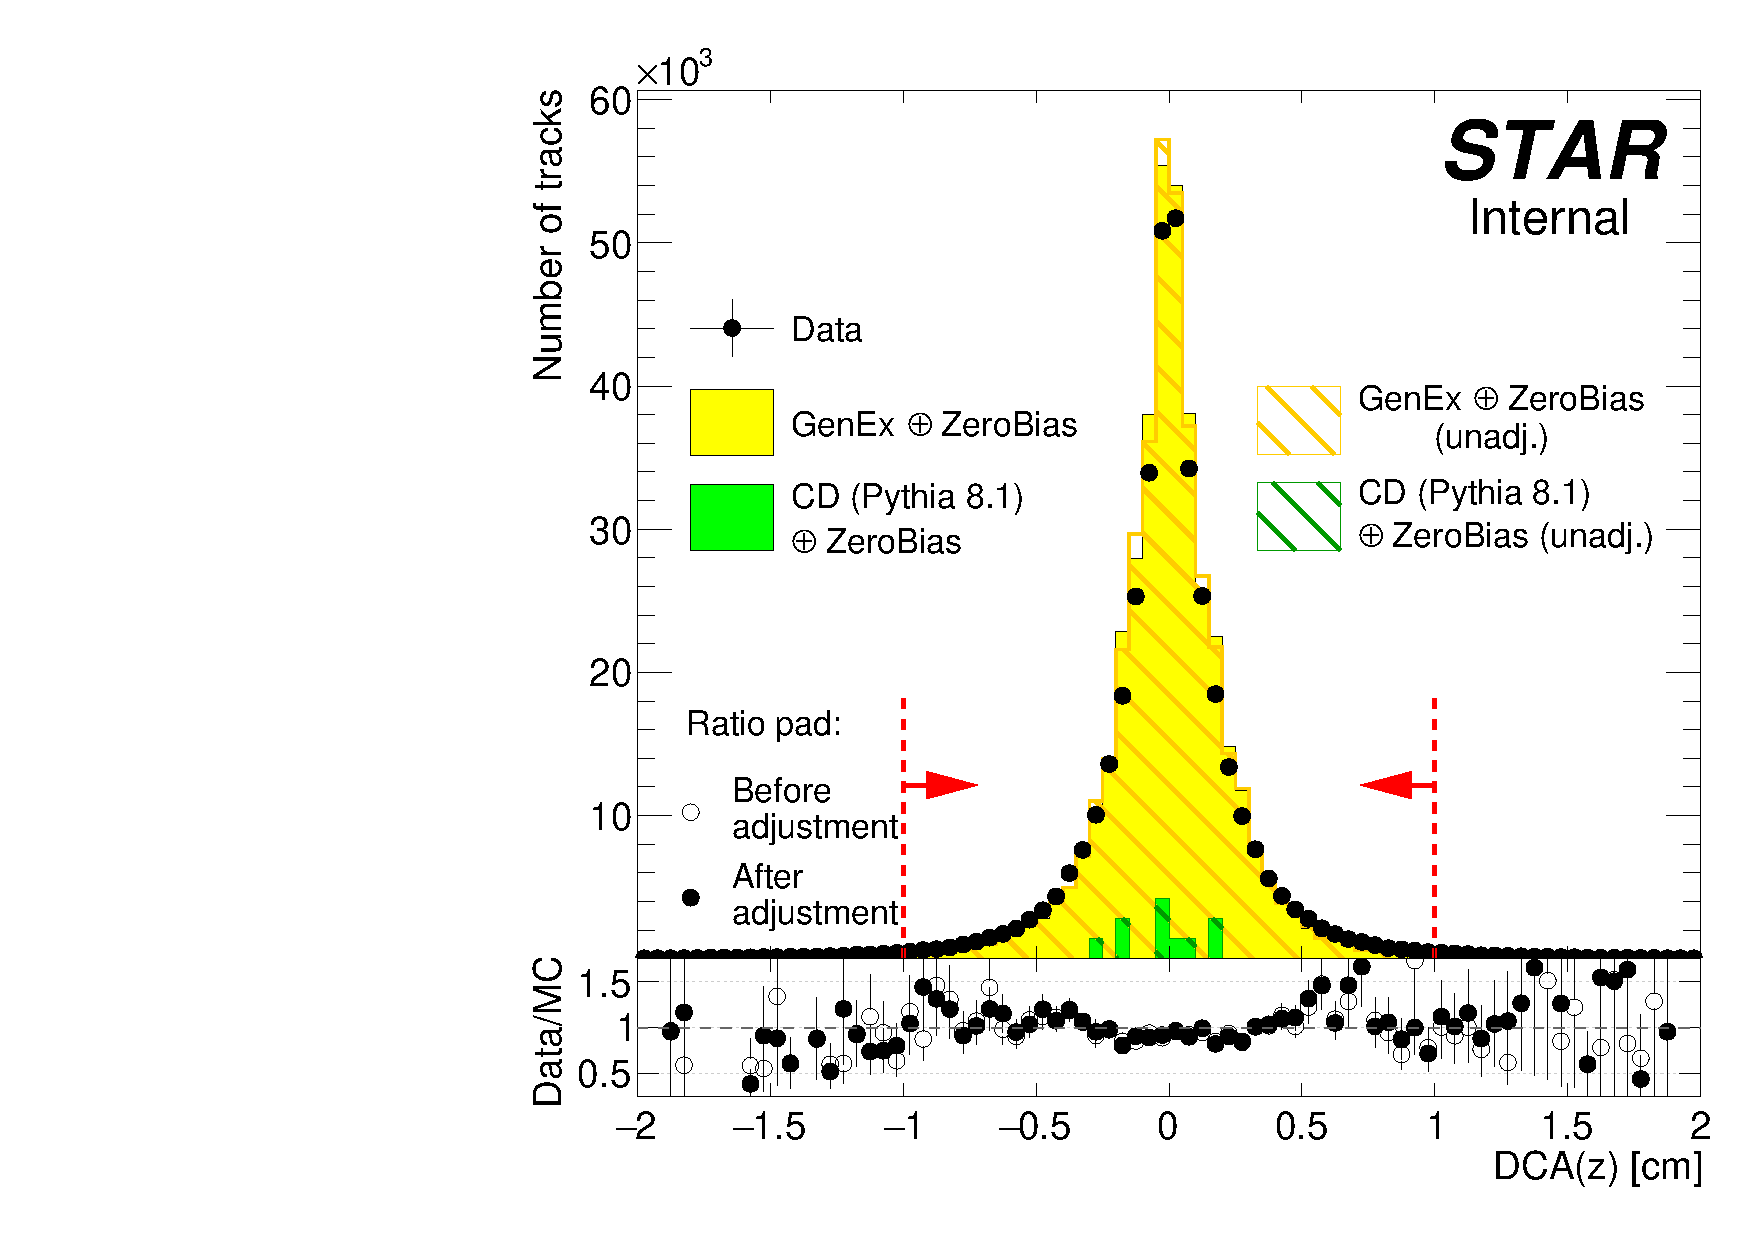
\includegraphics[width=\linewidth]{graphics/tpcHelixAdj/LongitudinalDCA_beforeAfterCorrection.pdf}}
  \end{subfigure}
}%
\quad\quad%
\parbox{0.4725\textwidth}{
  \centering
  \begin{subfigure}[b]{\linewidth}\addtocounter{subfigure}{-4}
                \subcaptionbox{\label{fig:dcaR}}{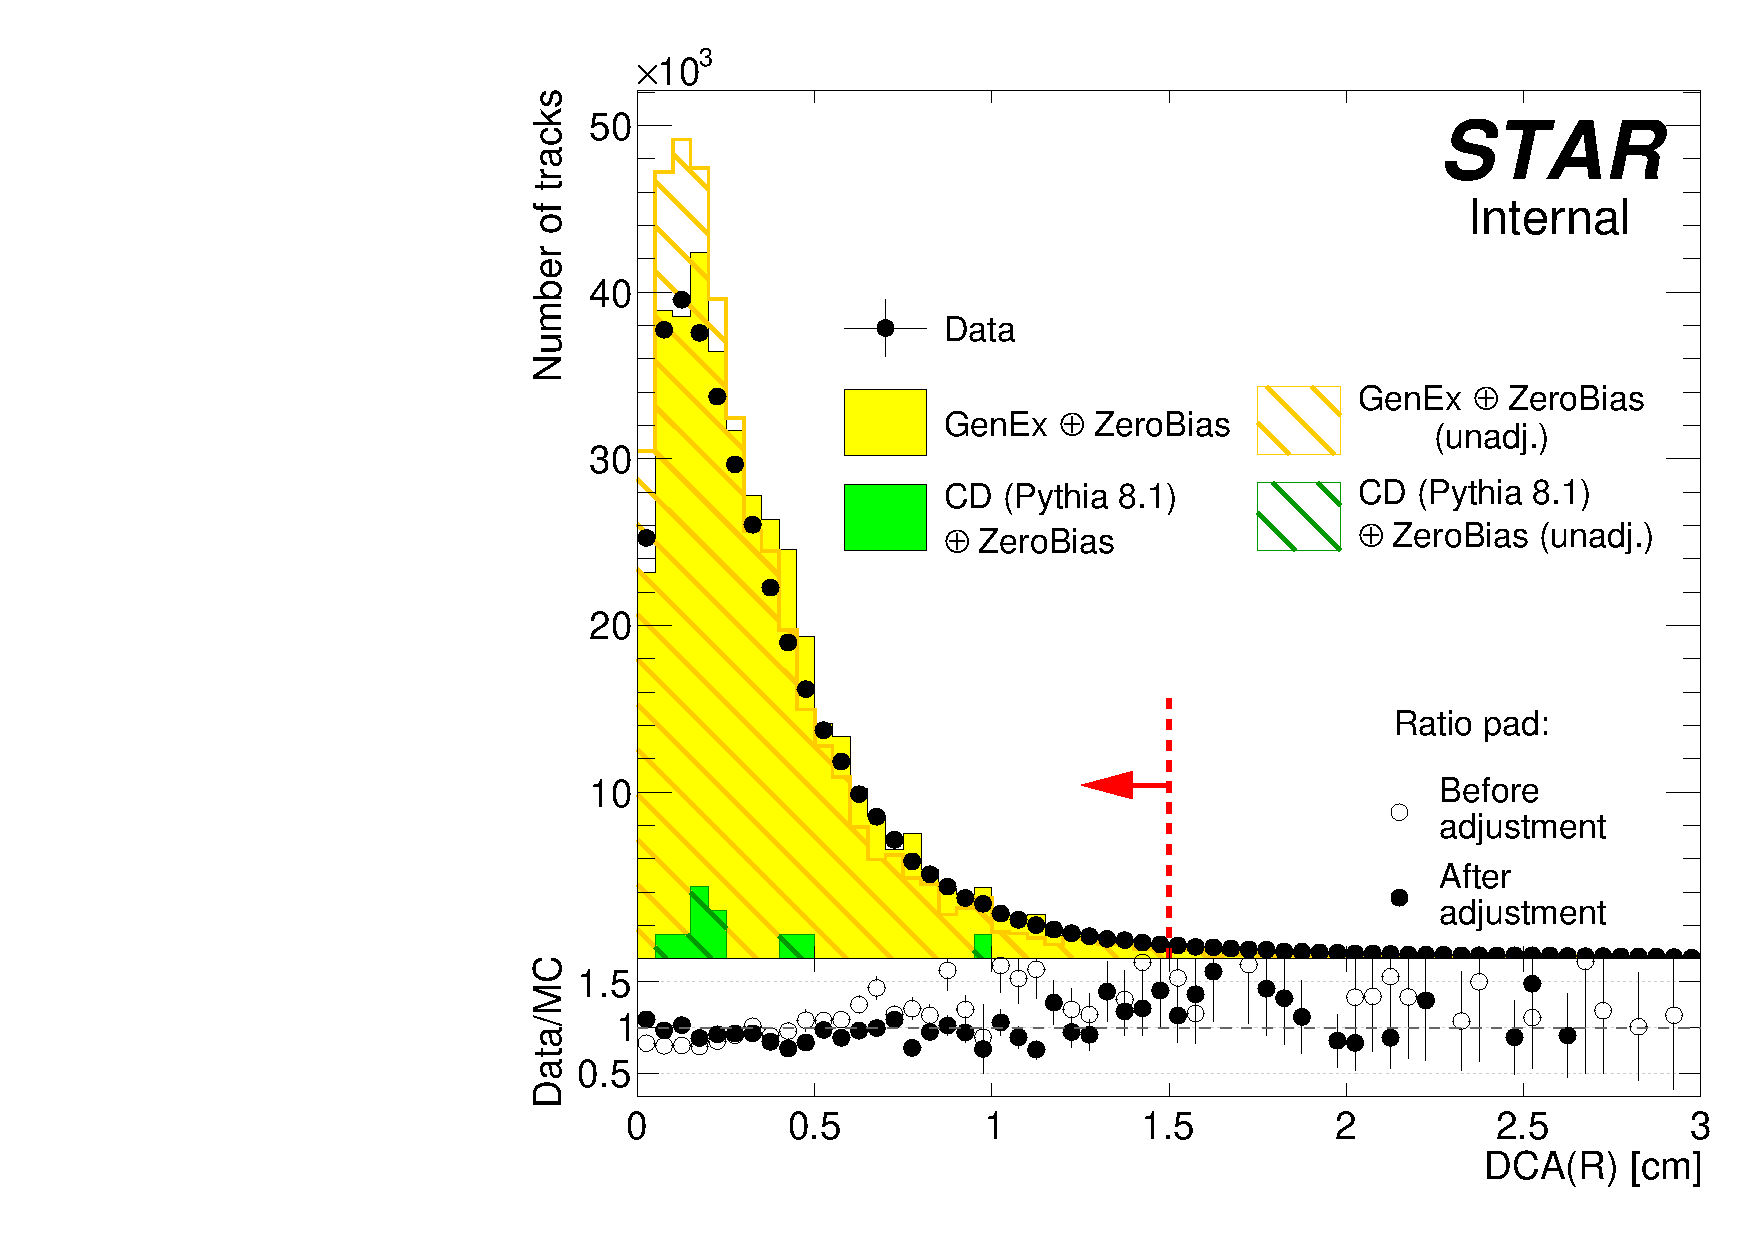
\includegraphics[width=\linewidth]{graphics/tpcHelixAdj/RadialDCA_beforeAfterCorrection.pdf}}
  \end{subfigure}\\
  \begin{subfigure}[b]{\linewidth}\addtocounter{subfigure}{1}
                \subcaptionbox{\label{fig:dcaY}}{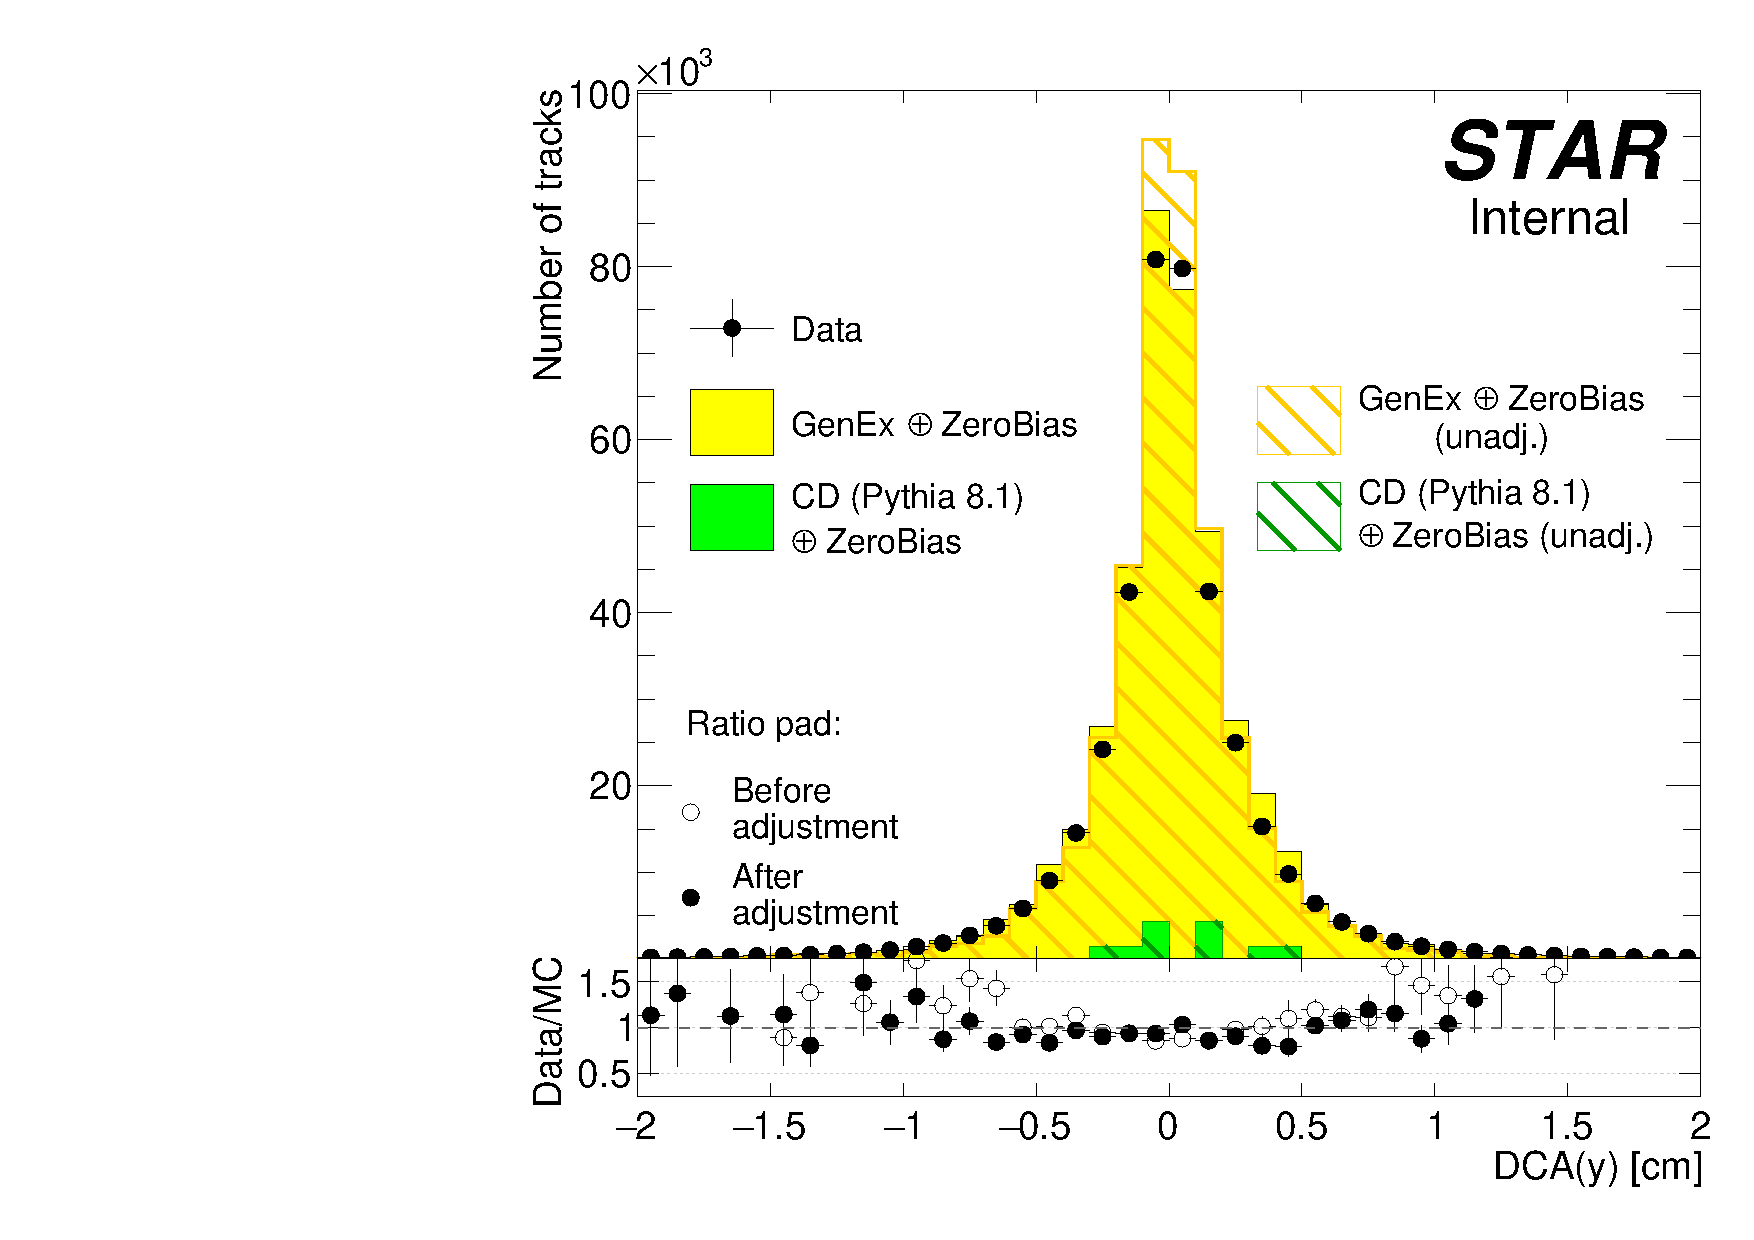
\includegraphics[width=\linewidth]{graphics/tpcHelixAdj/DcaY_beforeAfterCorrection.pdf}}
  \end{subfigure}
  \begin{minipage}[t][1.042\linewidth][t]{\linewidth}\vspace{10pt}
    \caption[Comparison of distribution of pion $d_{0}$ and components of DCA vector in the data and embedded MC, before and after adjustment of TPC pointing resolution.]
    {Comparison of distribution of pion transverse impact parameter $d_{0}$~(\ref{fig:d0}) and transverse~(\ref{fig:dcaR}), $x$-~(\ref{fig:dcaX}), $y$-~(\ref{fig:dcaY}) and $z$-component (\ref{fig:dcaZ}) of the DCA vector between the global helix and primary vertex in the data (CEP) and embedded MC (GenEx). Distributions for unadjusted helices are drawn as hashed histograms, while filled histograms are for adjusted helices. Normalizations of the signal and backgrounds were established from the comparison of $p_{T}^{\textrm{miss}}$ and $\Delta\theta$ distributions after full selection (without cut on the presented quantity and without exclusivity cut), as described in Sec.~XXX of~Ref.~\cite{AnalysisNoteRafal}. Red dashed lines and red arrows indicate the range of each quantity which is accepted in analyses.}\label{fig:pointingResComp}
  \end{minipage}
}%

\end{figure}
%---------------------------
